\documentclass{beamer}

\usepackage[utf8]{inputenc}
\usepackage{ngerman}
\usepackage[ngerman]{babel}


% Theme
\usetheme{metropolis}

% eckige bullets
\setbeamertemplate{items}[square]

% eckige bullets in table of content
\setbeamertemplate{section in toc}[square]

%\setbeamertemplate{frame footer}{\color{gray} Anna Scholtz $\|$ Linear Regression}

\usepackage{minted}

\usepackage{listings}

\usepackage[many]{tcolorbox}

\usepackage{tikz}
\usetikzlibrary{shadows,calc}



% Anführungszeichen: Genau, dies ist \enquote{nur} ein Beispiel.
\usepackage[babel,german=quotes]{csquotes}

\newcommand{\specialcell}[2][l]{%
  \begin{tabular}[#1]{@{}l@{}}#2\end{tabular}}

\beamertemplatenavigationsymbolsempty

% Pfeilsymbole
\usepackage{pifont}

% Pfeil unten rechts
\newcommand{\pfeil}{\ding{229}}


% zum Bilder einfügen
\usepackage{graphicx}
\usepackage{subfig}

% Fußnote ohne Nummer
\newcommand{\footnoteon}[1]{\let\thefootnote\relax\footnotetext{\tiny #1}}

% custom item bullets
%\newcommand*\pro{\item[{\includegraphics[height=1.6ex]{images/pro.pdf}}]}
%\newcommand*\con{\item[{\includegraphics[height=1.6ex]{images/con.pdf}}]}


% Inhaltsverzeichniss bis zur zweiten Ebene anzeigen
\setcounter{tocdepth}{1}

%\setbeamertemplate{footline}[frame number]

\newcommand{\ssec}[1]{\textbf{\Large #1} \hfill}

%7
\setbeamercovered{transparent=20}

% \AtBeginSubsection[]{
%     \begin{frame}<beamer>
%         \frametitle{Outline}
%         \tableofcontents[currentsection, currentsubsection]
%     \end{frame}
% }
%
% \AtBeginSection[]{
%     \begin{frame}<beamer>
%         \frametitle{Outline}
%         \tableofcontents[currentsection,currentsubsection]
%     \end{frame}
% }

\newcommand{\btVFill}{\vskip0pt plus 1filll}
\setbeamertemplate{subsection in toc}{\hspace*{2em}\inserttocsectionnumber.\inserttocsubsectionnumber.~\inserttocsubsection\par}

\setbeamercolor{pp}{
    bg=block title.bg!50!normal text.bg
  }




% some parameters for customization
\def\shadowshift{3pt,-3pt}
\def\shadowradius{6pt}

\colorlet{innercolor}{black!40}
\colorlet{outercolor}{gray!05}

% this draws a shadow under a rectangle node
\newcommand\drawshadow[1]{
    \begin{pgfonlayer}{shadow}
        \shade[outercolor,inner color=innercolor,outer color=outercolor] ($(#1.south west)+(\shadowshift)+(\shadowradius/2,\shadowradius/2)$) circle (\shadowradius);
        \shade[outercolor,inner color=innercolor,outer color=outercolor] ($(#1.north west)+(\shadowshift)+(\shadowradius/2,-\shadowradius/2)$) circle (\shadowradius);
        \shade[outercolor,inner color=innercolor,outer color=outercolor] ($(#1.south east)+(\shadowshift)+(-\shadowradius/2,\shadowradius/2)$) circle (\shadowradius);
        \shade[outercolor,inner color=innercolor,outer color=outercolor] ($(#1.north east)+(\shadowshift)+(-\shadowradius/2,-\shadowradius/2)$) circle (\shadowradius);
        \shade[top color=innercolor,bottom color=outercolor] ($(#1.south west)+(\shadowshift)+(\shadowradius/2,-\shadowradius/2)$) rectangle ($(#1.south east)+(\shadowshift)+(-\shadowradius/2,\shadowradius/2)$);
        \shade[left color=innercolor,right color=outercolor] ($(#1.south east)+(\shadowshift)+(-\shadowradius/2,\shadowradius/2)$) rectangle ($(#1.north east)+(\shadowshift)+(\shadowradius/2,-\shadowradius/2)$);
        \shade[bottom color=innercolor,top color=outercolor] ($(#1.north west)+(\shadowshift)+(\shadowradius/2,-\shadowradius/2)$) rectangle ($(#1.north east)+(\shadowshift)+(-\shadowradius/2,\shadowradius/2)$);
        \shade[outercolor,right color=innercolor,left color=outercolor] ($(#1.south west)+(\shadowshift)+(-\shadowradius/2,\shadowradius/2)$) rectangle ($(#1.north west)+(\shadowshift)+(\shadowradius/2,-\shadowradius/2)$);
        \filldraw ($(#1.south west)+(\shadowshift)+(\shadowradius/2,\shadowradius/2)$) rectangle ($(#1.north east)+(\shadowshift)-(\shadowradius/2,\shadowradius/2)$);
    \end{pgfonlayer}
}

% create a shadow layer, so that we don't need to worry about overdrawing other things
\pgfdeclarelayer{shadow}
\pgfsetlayers{shadow,main}


\newcommand\shadowimage[2][]{%
\begin{tikzpicture}
\node[anchor=south west,inner sep=0] (image) at (0,0) {\includegraphics[#1]{#2}};
\drawshadow{image}
\end{tikzpicture}}




\begin{document}



\title[Verifying the Rope datastructure of Xi-Editor]{Verifying the Rope Data Structure of Xi-Editor}

\author{Anna Scholtz}
%\institute[TU Chemnitz]{TU Chemnitz}




\frame[plain]{
    \titlepage
}


\frame{
    \frametitle{Outline}\tableofcontents[]

}


\section{Motivation}

\begin{frame}{Goal and Motivation}
  \begin{itemize}
    \item \textbf{Motivation:} Need for good text editors
    \begin{itemize}
      \item Xi-editor: combines newer concepts for storing text to allow very high performance
      \item Core idea: modified rope data structure for storing text as well as edit history
    \end{itemize}
    \item \textbf{Goal:} Verification of the rope data structure in xi-editor  %[why?]
  \end{itemize}
\end{frame}


\section{Background}

\subsection{Xi-Editor}

\begin{frame}{Xi-Editor}
    \begin{figure}
        \centering
        
\includegraphics[width=8cm]{images/xi-github.png}
    \end{figure}
\end{frame}


\subsection{Rope Data Structures}

\begin{frame}{Rope Data Structures}
  \begin{columns}
    \begin{column}{0.5\textwidth}
        \begin{itemize}
            \item Binary Tree
            \item Only leaves contain text
            \item Operations: Index, Split, Concatenate, Report, Insert, Delete
        \end{itemize}
    \end{column}
    \begin{column}{0.5\textwidth}
      \begin{figure}
          \centering
          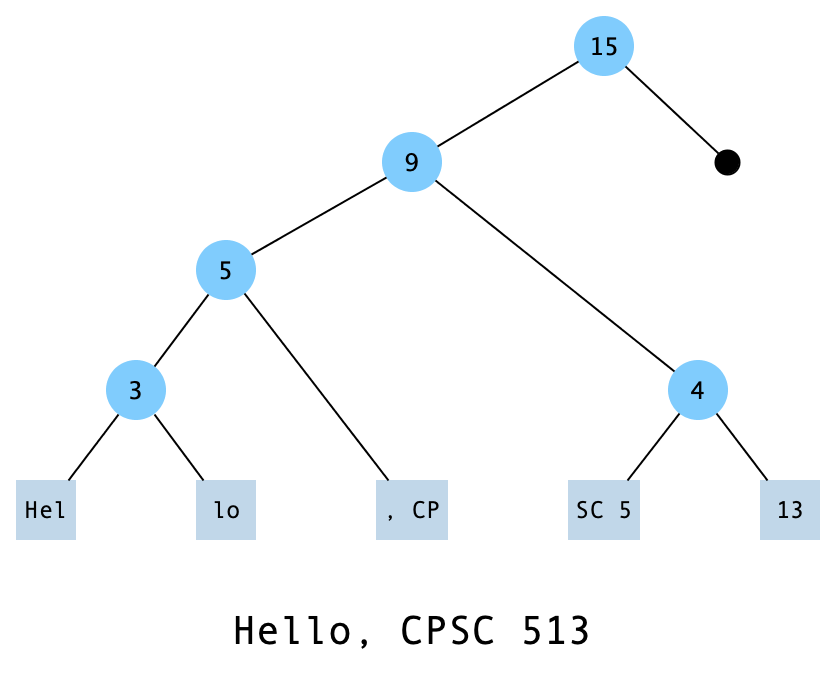
\includegraphics[width=5.5cm]{images/rope.png}
      \end{figure}
    \end{column}
  \end{columns}
\end{frame}





\subsection{Rope Data Structure in Xi-Editor}

\begin{frame}{Rope Data Structure in Xi-Editor}
  \begin{itemize}
      \item B-Tree
      \item Operations: Concatenate, Slice, Insert, SliceToString
  \end{itemize}
  \begin{figure}
      \centering
      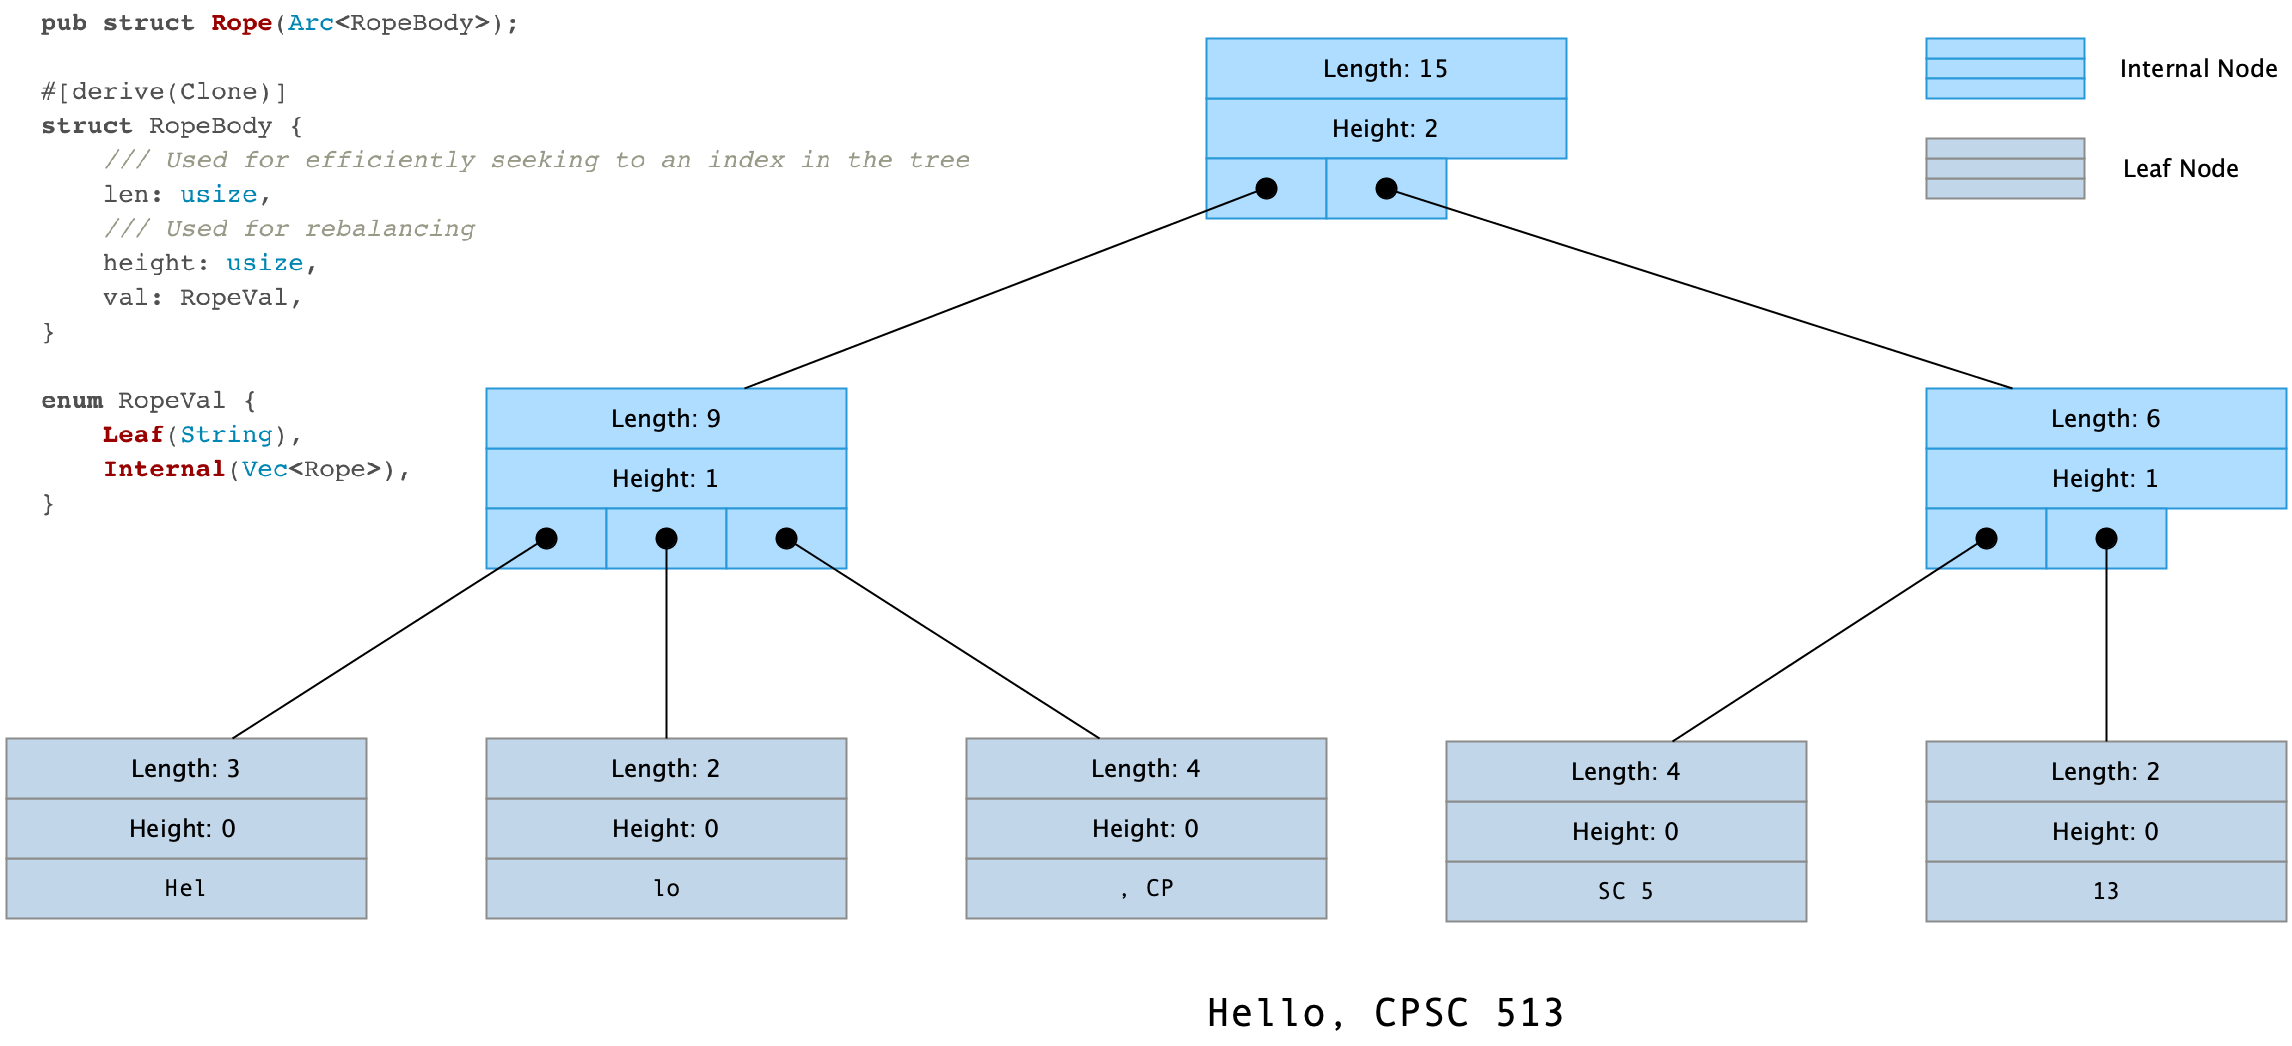
\includegraphics[width=11cm]{images/xi-rope.png}
  \end{figure}

  \btVFill

  \tiny{\url{https://github.com/xi-editor/xi-editor/blob/master/rust/rope/src/tree.rs}}
  \smallskip
\end{frame}


\section{Verifying Ropes}

\begin{frame}{Verifying Ropes}
  \begin{itemize}
      \item \textbf{Goal:}
        \begin{itemize}
          \item Define properties of ropes
          \item Verify that after applying operations, these properties still hold
          \item Verify that this also works for distributed ropes (collaborative editing)
        \end{itemize}
      \item Approach: first verify standard rope data structure (simpler), then verify rope data structure of xi-editor
  \end{itemize}
\end{frame}

\subsection{Dafny}

\begin{frame}{Dafny}
  \begin{columns}
    \begin{column}{0.5\textwidth}
        \begin{itemize}
            \item Language and verifier
            \item Supports verification through pre-conditions, post-conditions, loop invariants, ...
            \item Dafny programs are translated into Boogie 2 which is used to generate first-order verification conditions that are passed to the SMT solver Z3
        \end{itemize}
    \end{column}
    \begin{column}{0.5\textwidth}
      \begin{figure}
          \centering
          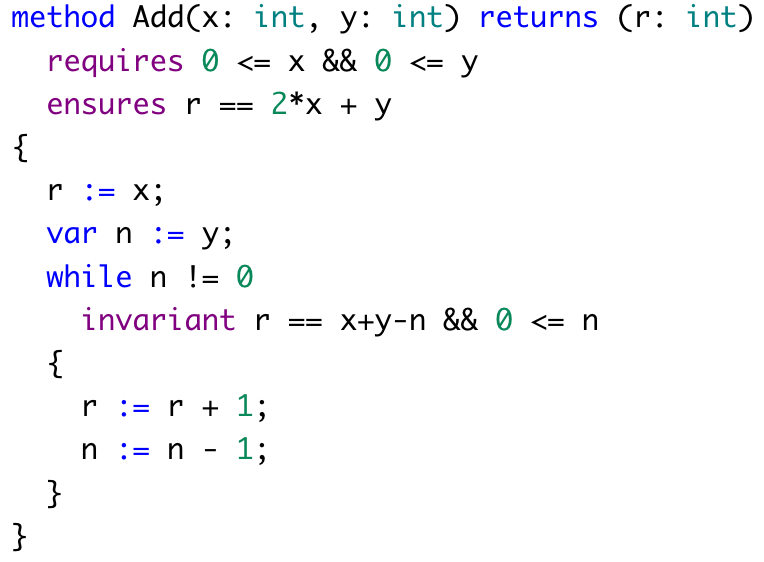
\includegraphics[width=5.5cm]{images/dafny.png}
      \end{figure}
    \end{column}
  \end{columns}
\end{frame}

\subsection{Properties Standard Rope}

\begin{frame}{Properties Standard Rope}
    \begin{enumerate}
        \item Every node has at most two children
        \item Only leaves contain data
        \item Weight values of non-leaf nodes is the length of all children in the left subtree
        \item Weight values of leaf nodes is the length of the stored text
    \end{enumerate}
\end{frame}


\subsection{Standard Rope Verification}

\begin{frame}{Standard Rope Verification}
  Rope Data Structure:

  \begin{figure}
      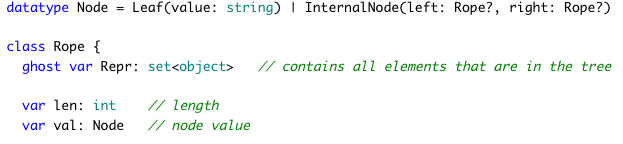
\includegraphics[width=8.5cm]{images/rope-datastructure.png}
  \end{figure}

  Validity Conditions:

  \begin{figure}
      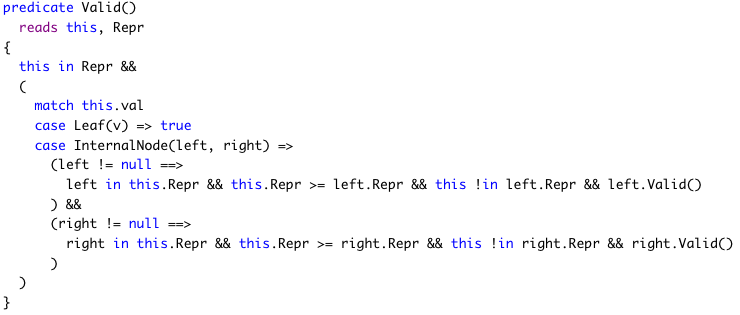
\includegraphics[width=9.5cm]{images/rope-valid.png}
  \end{figure}

\end{frame}

\begin{frame}{Standard Rope Verification}
  Validity Conditions:

  \begin{figure}
      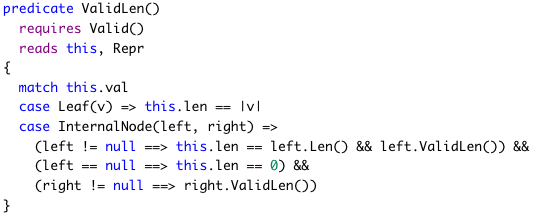
\includegraphics[width=8.5cm]{images/rope-valid-len.png}
  \end{figure}

\end{frame}

\begin{frame}{Standard Rope Verification}
  Implemented Methods:

  \begin{figure}
    \begin{tabular}{ll}
      \subfloat{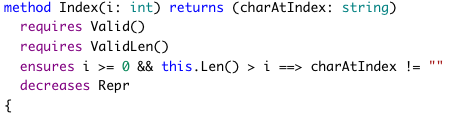
\includegraphics[width=6cm]{images/rope-index.png}} \\
      % \subfloat{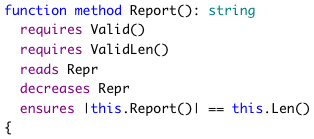
\includegraphics[width=4.5cm]{images/rope-report.png}} \\
      % \subfloat{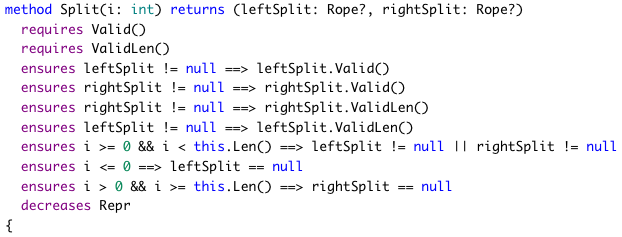
\includegraphics[width=5.5cm]{images/rope-split.png}} &
      \subfloat{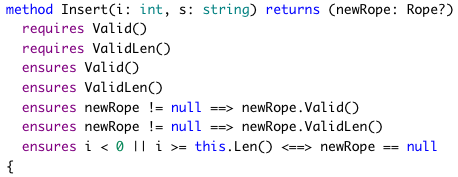
\includegraphics[width=6cm]{images/rope-insert.png}} \\
      \subfloat{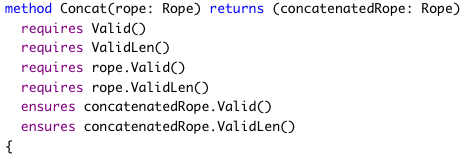
\includegraphics[width=6cm]{images/rope-concat.png}} \\
      % \subfloat{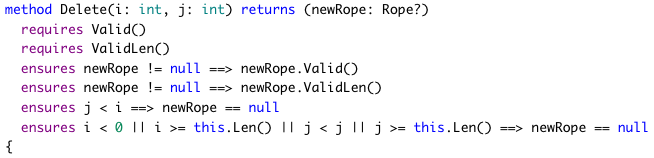
\includegraphics[width=5cm]{images/rope-delete.png}} \\
    \end{tabular}
  \end{figure}
\end{frame}



\subsection{Properties Xi-Editor Rope}

\begin{frame}{Properties Xi-Editor Rope}
  \begin{enumerate}
      \item Every node has at most $MAX\_CHILDREN$ children
      \item Every non-leaf node, except the root node, has at least $MIN\_CHILDREN$ child nodes
      \item The root has at least two children if it is not a leaf node
      \item Only leaves contain data
      \item The length of the text stored in leaf nodes is at most $MAX\_LEAF$
      \item Weight values of non-leaf nodes is the sum of the children's weights
      \item Weight values of leaf nodes is the length of the stored text
      \item All leaves appear in the same level
  \end{enumerate}
\end{frame}


\subsection{Xi-Editor Rope Verification}

\begin{frame}{Xi-Editor Rope Verification}
  Rope Data Structure:

  \begin{figure}
      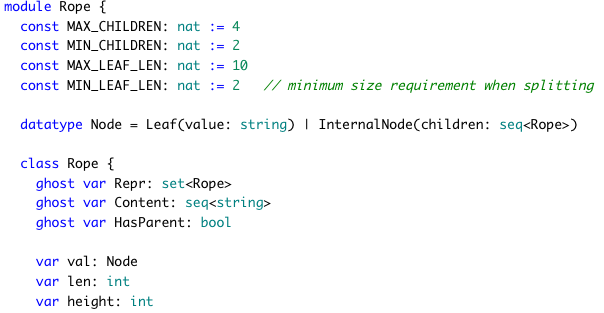
\includegraphics[width=9.5cm]{images/xi-rope-datastructure.png}
  \end{figure}
\end{frame}

\begin{frame}{Xi-Editor Rope Verification}
  Validity Conditions:

  \begin{figure}
      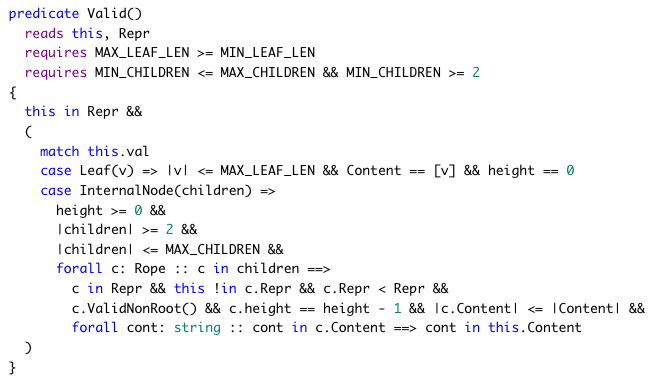
\includegraphics[width=10.5cm]{images/xi-rope-valid.png}
  \end{figure}

\end{frame}


\begin{frame}{Xi-Editor Rope Verification}
  Validity Conditions:

  \begin{figure}
      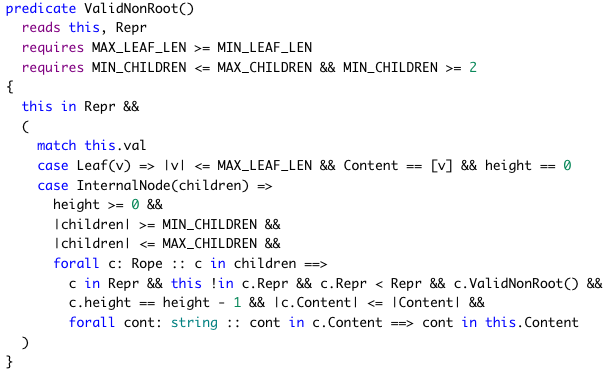
\includegraphics[width=10cm]{images/xi-rope-non-valid-root.png}
  \end{figure}

\end{frame}

\begin{frame}{Xi-Editor Rope Verification}
  Validity Conditions:

  \begin{figure}
      \centering
      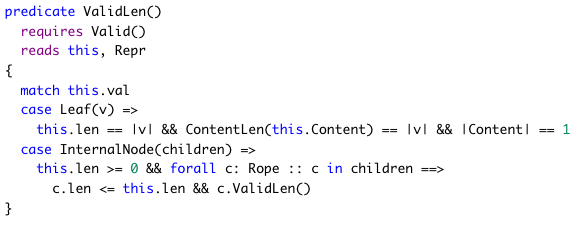
\includegraphics[width=9.5cm]{images/xi-rope-valid-len.png}
  \end{figure}
\end{frame}

\begin{frame}{Xi-Editor Rope Verification}
  Implemented Methods (work in progress):

  \begin{figure}
    \begin{tabular}{ll}
      \subfloat{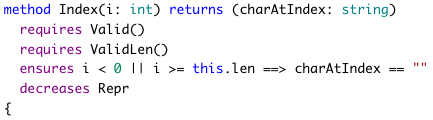
\includegraphics[width=6.5cm]{images/xi-rope-index.png}} \\
      \subfloat{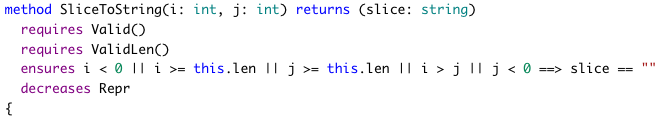
\includegraphics[width=9.5cm]{images/xi-rope-slice-to-string.png}} \\
    \end{tabular}
  \end{figure}
\end{frame}


\section{Future Work}


\begin{frame}{Future Work}
  \begin{itemize}
    \item Implement remaining methods for xi-editor rope
    \item Implement transactions and verify that properties hold in a collaborative environment (out-of-scope)
    \item Verify other parts of xi-editor (very much out-of-scope)
  \end{itemize}

\end{frame}






\end{document}
